\documentclass{article}
\usepackage[utf8]{inputenc}
\usepackage[brazil]{babel}
\usepackage{epsfig}
\usepackage{fancyhdr}
\usepackage{indentfirst} %In­dent first para­graph af­ter sec­tion header
\usepackage{titlesec}
\usepackage{amsmath}
\usepackage{amsthm}

\pagestyle{empty}

\headheight 40mm      %
\oddsidemargin 2.0mm  %
\evensidemargin 2.0mm %
\topmargin -40mm      %
\textheight 250mm     %
\textwidth 160mm      %
%
\newcounter{execs}
\setcounter{execs}{0}
\newcommand{\exec}[0]{\addtocounter{execs}{1}\item[\textbf{\arabic{execs}.}]}

\fancypagestyle{first}
{
\pagestyle{fancy}
}
%%%%%%%%%%%%%%%%%%%%%%%%%%%%%%%%%%%%%%%%%%%%%%%%%%%%%%%%
%%%%%%%%%%%%%%%%%%%%%%%%%%%%%%%%%%%%%%%%%%%%%%%%%%%%%%%%
% PLEASE, EDIT THIS!
\fancyhead[LO]{\small Trabalho \\ 
                DCC008 - Cálculo Numérico  \\
                \textbf{Entrega: 09 de Dezembro de 2018} }

\fancyhead[RO]{\small Universidade Federal de Juiz de Fora - UFJF \\ 
                Departamento de Ciência da Computação \\
               \textit{Nome: Thiago de Almeida}\\
               \textit{Nome: Renan Nunes}}


\begin{document}
\thispagestyle{first}
    \noindent \textbf{Obs1.:}  Em todos os casos utilize integração numérica com $n+1$ pontos, onde $n$ é a ordem do polinômio empregado na aproximação por elementos finitos.
    
    \noindent \textbf{Obs2.:} Apresente gráficos separados para cada caso estudado, menos para o item (e).

    \noindent \textbf{Obs3.:} declare as variáveis utilizando a máxima precisão possível.
\begin{itemize}

\exec Seja o problema de difusão-reação:
\begin{align} \label{prob1}
- \varepsilon\dfrac{d^2 u}{d x^2} + u &= 1, \quad x\in \Omega= [0,1]
 \\ \label{cc1}
 u(0)&=u(1)=0.
\end{align}
A solução exata para o problema \eqref{prob1}-\eqref{cc1} é
\begin{equation}\label{solexat1}
u(x) = c_1 e^{-\tfrac{x}{\sqrt{\varepsilon}}} + c_2 e^{\tfrac{x}{\sqrt{\varepsilon}}}+1
\end{equation}
onde $c_1 = -1-c_2$ e $c_2 = \dfrac{e^{-\tfrac{1}{\sqrt{\varepsilon}}}-1}
{e^{\tfrac{1}{\sqrt{\varepsilon}}}-e^{-\tfrac{1}{\sqrt{\varepsilon}}}}$. 

A partir de uma aproximação do problema \eqref{prob1}-\eqref{cc1} pelo método de elementos finitos, faça:

\begin{itemize}
  
\item[a)] Compare a solução exata e a aproximado para:
\begin{itemize}
\item $\varepsilon = 10^{-3}$ com $4$ e $8$ elementos;
\item $\varepsilon = 10^{-4}$ com $16$ e $32$ elementos; 
\end{itemize}
utilizando polinômios de primeira ordem ($n=1$).

\item[b)] Realizando uma análise da discretização 
gerada pelo método de elementos finitos do item (a) obtém-se 
a seguinte relação de estabilidade $h<\sqrt{6\varepsilon}$. Valide  
graficamente esta relação para $\varepsilon = 10^{-3}$ e $\varepsilon = 10^{-4}$.

\item[c)] Repita o item (a) utilizando polinômios de ordem $n =2,3,4,5$. 

\item[d)] Compare os resultados dos itens (a) e (c) com 
a aproximação obtida pelo método de 
diferenças finitas (Questão 2 da Lista 1) e a solução exata.

\item[e)] apresente um gráfico da taxa de convergência comparando o erro 
entre a solução exata e a aproximada tomando $\varepsilon = 10^{-3}$ 
para malhas formadas por $4^i$ elementos, 
com $i=1,2,3,4,5$, utilizando a norma do máximo ou L2 
para aproximações por elementos finitos de ordem $n=1,2,3,4,5$ e diferenças finitas 
(apresente todos os resultados no mesmo gráfico). 

\end{itemize}

\end{itemize}

\newpage


Para resolução da Lista 7 foram utilizados os métodos implementados em listas anteriores de forma a elaborar uma função resolução de elementos finitos.
Todos os gráficos e métodos foram gerados com máxima precisão possível, float128.

\begin{itemize}
\item [a)] Comparação da solução exata com a solução aproximada, com polinomios $n=1$:
\begin{itemize}
\item $\varepsilon = 10^{-3}$ com $4$ e $8$ elementos;

\begin{figure}[!htb]
\centering
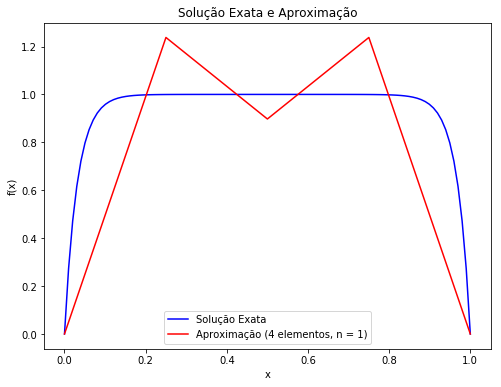
\includegraphics[width=6cm,height=6cm]{LetraA/4el_n1_e10-3.png}
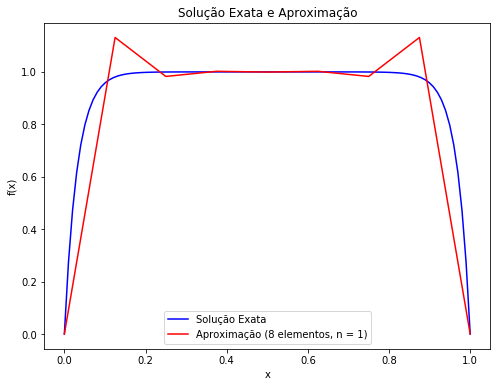
\includegraphics[width=6cm,height=6cm]{LetraA/8el_n1_e10-3.png}
\end{figure}

\item $\varepsilon = 10^{-4}$ com $16$ e $32$ elementos;

\begin{figure}[!htb]
\centering
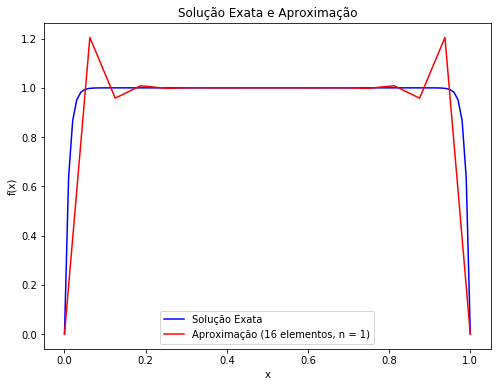
\includegraphics [width=6cm,height=6cm]{LetraA/16el_n1_e10-4.png}
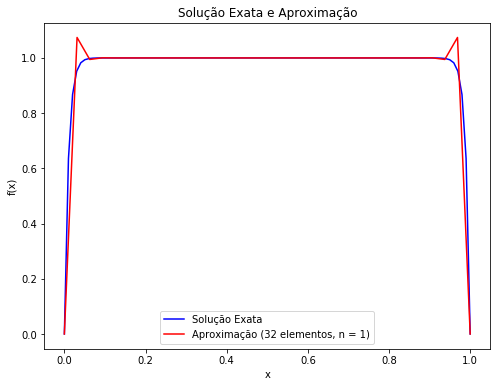
\includegraphics [width=6cm,height=6cm]{LetraA/32el_n1_e10-4.png}
\end{figure}

\end{itemize}

\newpage
\item[b)] Utilizando a discretização do item a, obtem-se a seguinte relação graficamente:

\begin{figure}[!htb]
\centering
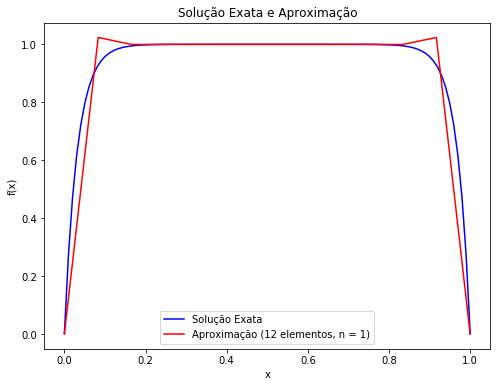
\includegraphics [width=6cm,height=6cm]{LetraB/12el_n1_e10-3.png}
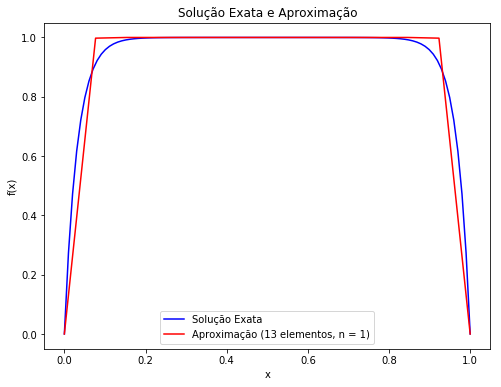
\includegraphics [width=6cm,height=6cm]{LetraB/13el_n1_e10-3.png}
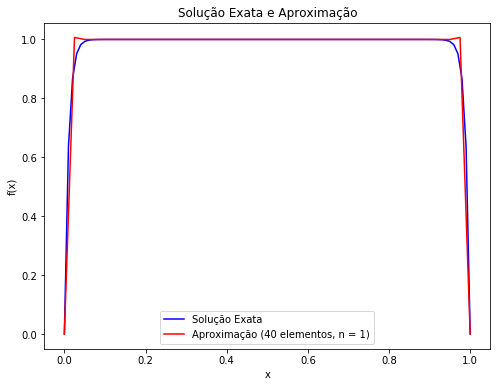
\includegraphics [width=6cm,height=6cm]{LetraB/40el_n1_e10-4.png}
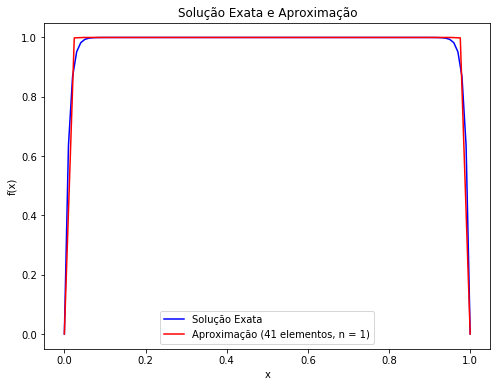
\includegraphics [width=6cm,height=6cm]{LetraB/41el_n1_e10-4.png}
\end{figure}

Assim, conclui-se que o metodo se torna estável em $nel>=13$, para $\varepsilon = 10^{-3}$\\
e $nel>=41$ para $\varepsilon = 10^{-4}$ evidenciado pela ausência do picos verticais nas extremidades superiores.

\newpage

\item[c)] Comparação da solução exata com a solução aproximada, com polinomios agora $n=2,3,4$ e $5$:
\begin{itemize}
\item Para n = 2.
\item $\varepsilon = 10^{-3}$ com $4$ e $8$ elementos;

\begin{figure}[!htb]
\centering
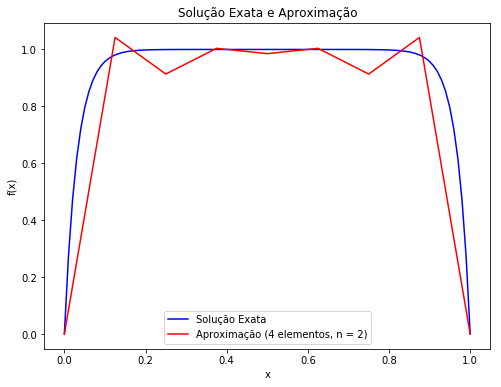
\includegraphics [width=6cm,height=6cm]{LetraC/4el_n2_e10-3.png}
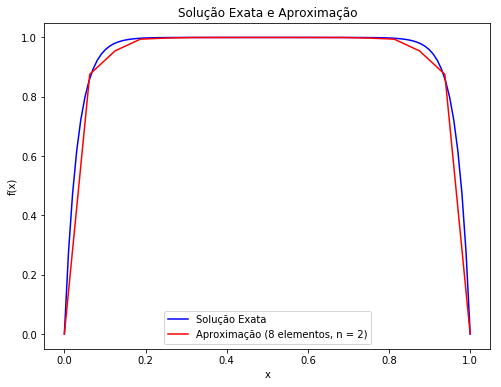
\includegraphics [width=6cm,height=6cm]{LetraC/8el_n2_e10-3.png}
\end{figure}

\item $\varepsilon = 10^{-4}$ com $4$ e $8$ elementos;

\begin{figure}[!htb]
\centering
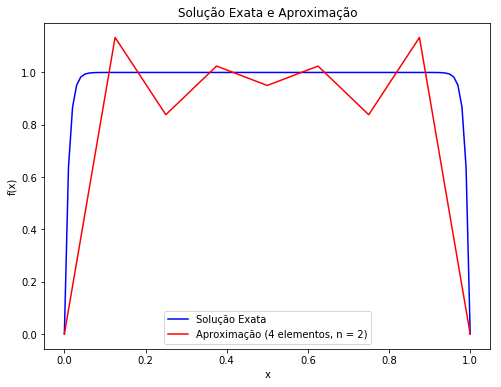
\includegraphics [width=6cm,height=6cm]{LetraC/4el_n2_e10-4.png}
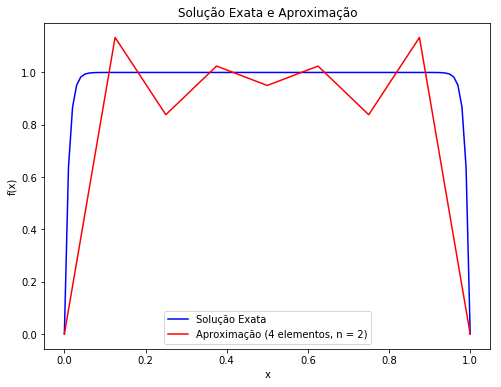
\includegraphics [width=6cm,height=6cm]{LetraC/4el_n2_e10-4.png}
\end{figure}

\newpage
\item Para n = 3.
\item $\varepsilon = 10^{-3}$ com $4$ e $8$ elementos;

\begin{figure}[!htb]
\centering
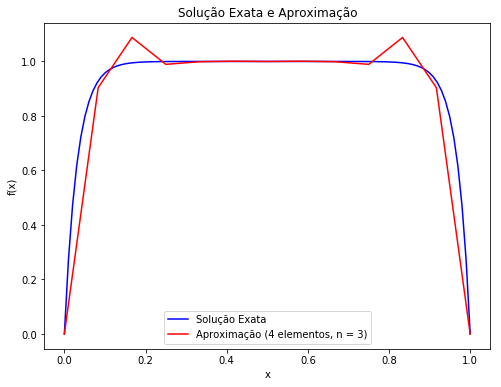
\includegraphics [width=6cm,height=6cm]{LetraC/4el_n3_e10-3.png}
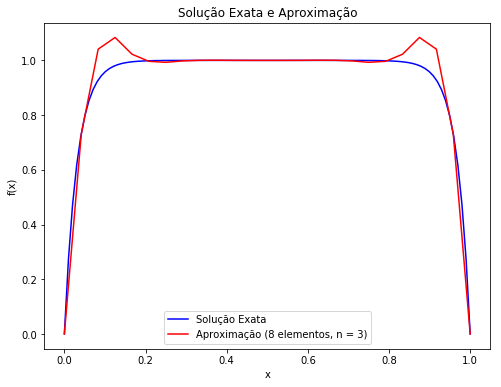
\includegraphics [width=6cm,height=6cm]{LetraC/8el_n3_e10-3.png}
\end{figure}

\item $\varepsilon = 10^{-4}$ com $16$ e $32$ elementos;

\begin{figure}[!htb]
\centering
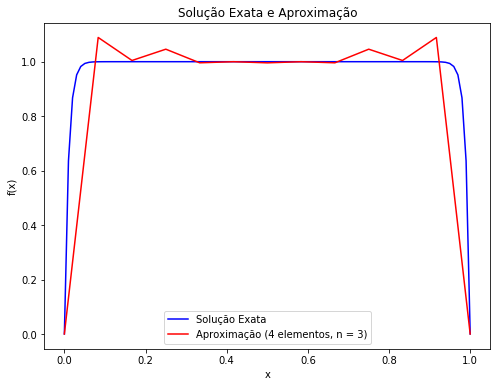
\includegraphics [width=6cm,height=6cm]{LetraC/4el_n3_e10-4.png}
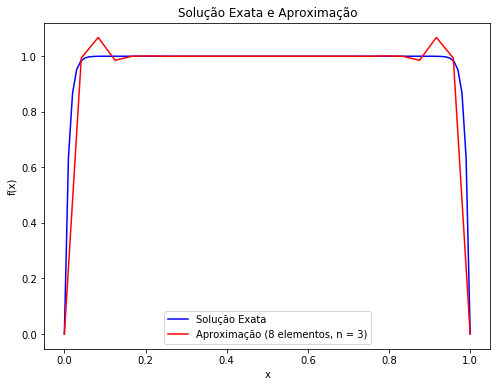
\includegraphics [width=6cm,height=6cm]{LetraC/8el_n3_e10-4.png}
\end{figure}

\newpage
\item Para n = 4.
\item $\varepsilon = 10^{-3}$ com $4$ e $8$ elementos;

\begin{figure}[!htb]
\centering
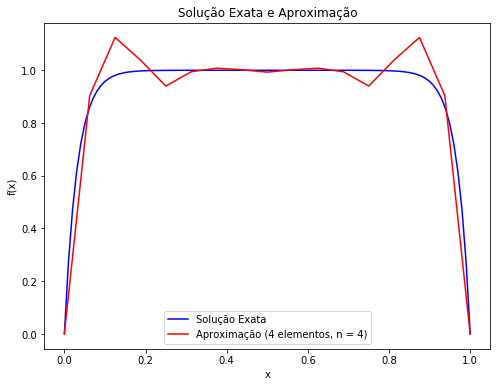
\includegraphics [width=6cm,height=6cm]{LetraC/4el_n4_e10-3.png}
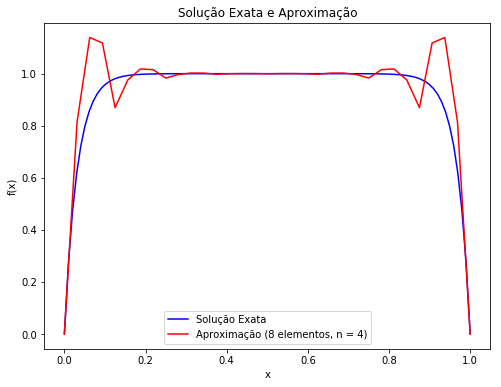
\includegraphics [width=6cm,height=6cm]{LetraC/8el_n4_e10-3.png}
\end{figure}

\item $\varepsilon = 10^{-4}$ com $16$ e $32$ elementos;

\begin{figure}[!htb]
\centering
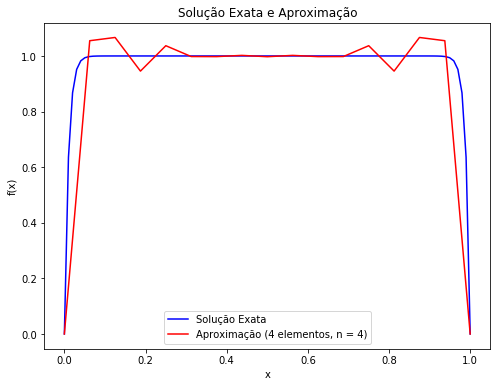
\includegraphics [width=6cm,height=6cm]{LetraC/4el_n4_e10-4.png}
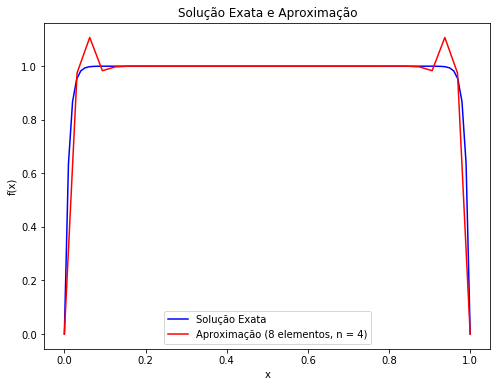
\includegraphics [width=6cm,height=6cm]{LetraC/8el_n4_e10-4.png}
\end{figure}

\newpage
\item Para n = 5.
\item $\varepsilon = 10^{-3}$ com $4$ e $8$ elementos;

\begin{figure}[!htb]
\centering
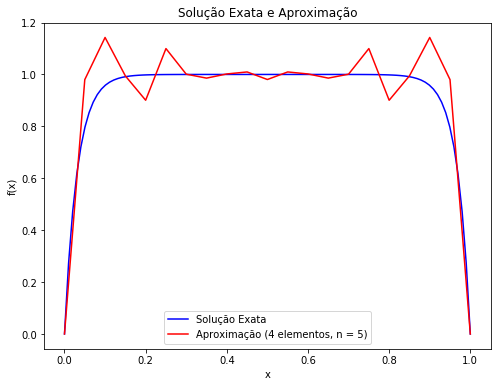
\includegraphics [width=6cm,height=6cm]{LetraC/4el_n5_e10-3.png}
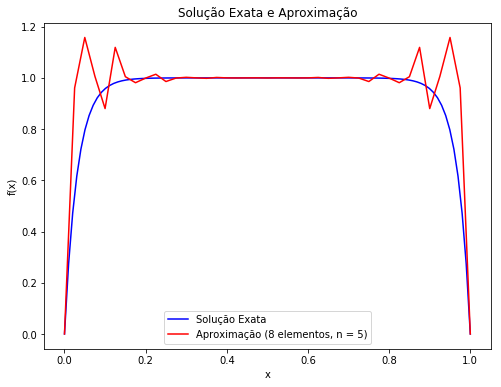
\includegraphics [width=6cm,height=6cm]{LetraC/8el_n5_e10-3.png}
\end{figure}

\item $\varepsilon = 10^{-4}$ com $16$ e $32$ elementos;

\begin{figure}[!htb]
\centering
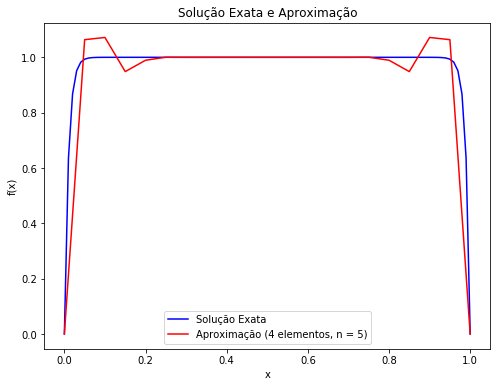
\includegraphics [width=6cm,height=6cm]{LetraC/4el_n5_e10-4.png}
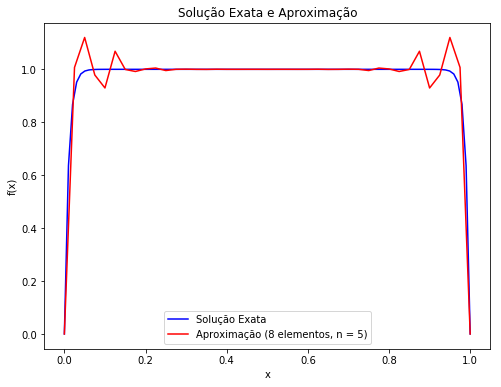
\includegraphics [width=6cm,height=6cm]{LetraC/8el_n5_e10-4.png}
\end{figure}

\end{itemize}

Conclui-se que o aumento da quantidade de elementos melhora a precisão do método de Elementos Finitos. Os picos presentes (instabilidades) também diminuem com o aumento da quantidade de elementos.

\newpage
\item[d)] Comparando os resultados do item a das listas 1 e 7.

\item $\varepsilon = 10^{-3}$ com $4$ elementos (Diferenças Finitas a esquerda, Elementos Finitos a direita);

\begin{figure}[!htb]
\centering
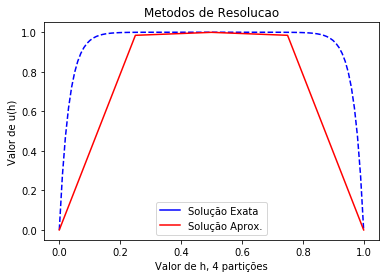
\includegraphics [width=5cm,height=5cm]{LetraD/4el_e10-3.png}
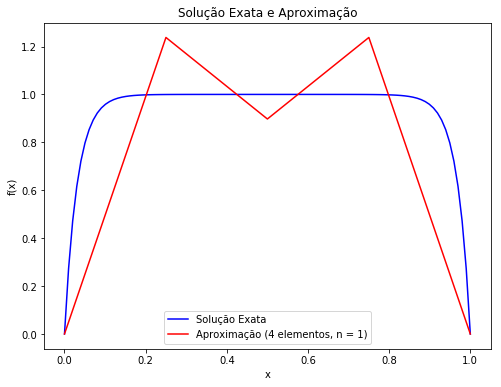
\includegraphics [width=5cm,height=5cm]{LetraA/4el_n1_e10-3.png}
\end{figure}

\item $\varepsilon = 10^{-3}$ com $8$ elementos (Diferenças Finitas a esquerda, Elementos Finitos a direita);

\begin{figure}[!htb]
\centering
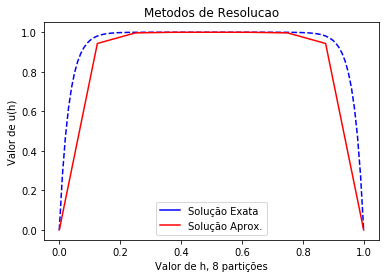
\includegraphics [width=5cm,height=5cm]{LetraD/8el_e10-3.png}
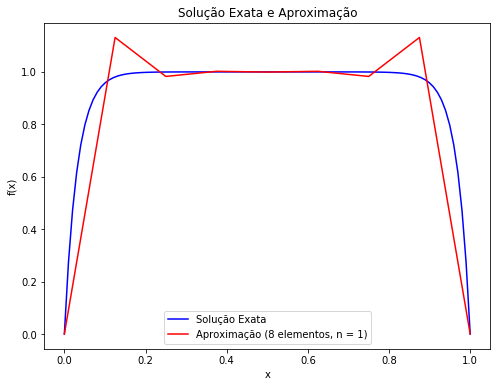
\includegraphics [width=5cm,height=5cm]{LetraA/8el_n1_e10-3.png}
\end{figure}

\newpage

\item $\varepsilon = 10^{-4}$ com $4$ elementos (Diferenças Finitas a esquerda, Elementos Finitos a direita);

\begin{figure}[!htb]
\centering
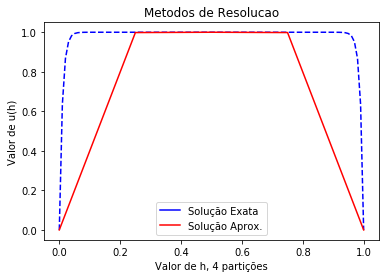
\includegraphics [width=5cm,height=5cm]{LetraD/4el_e10-4.png}
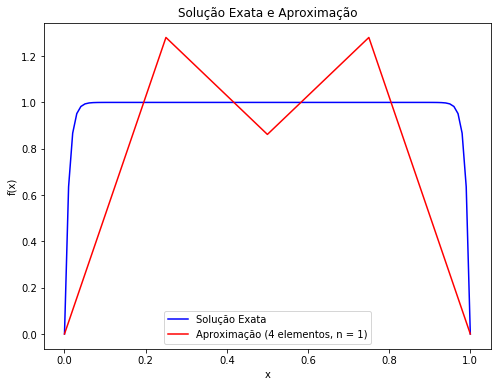
\includegraphics [width=5cm,height=5cm]{LetraD/4el_n1_e10-4.png}
\end{figure}

\item $\varepsilon = 10^{-4}$ com $8$ elementos (Diferenças Finitas a esquerda, Elementos Finitos a direita);

\begin{figure}[!htb]
\centering
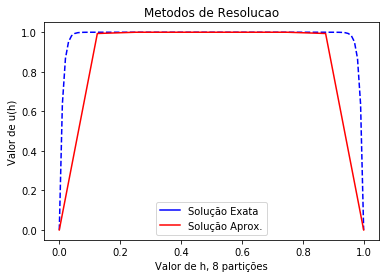
\includegraphics [width=5cm,height=5cm]{LetraD/8el_e10-4.png}
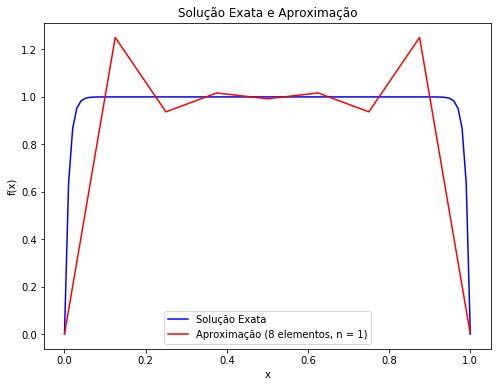
\includegraphics [width=5cm,height=5cm]{LetraD/8el_n1_e10-4.png}
\end{figure}

Conclusão: Nota-se que o método de Diferenças Finitas se comportou ligeiramente melhor em relação ao método de Elementos Finitos para o problema dado.

\newpage
\item[e)] A taxa de convergência da solução exata com o erro graficamente.

\begin{figure}[!htb]
\centering
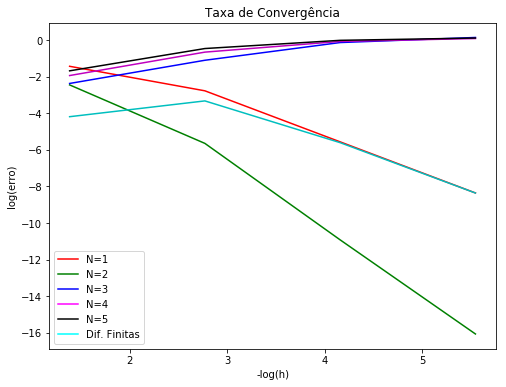
\includegraphics [width=12cm,height=9cm]{LetraE/taxa_convergencia.png}
\end{figure}

\end{itemize}

Conclusão final:

\end{document}
